\section{Příklad 2}
% Jako parametr zadejte skupinu (A-H)
\druhyZadani{C}

\section*{Riešenie}
\subsection*{1. krok}
Skratujeme napäťový napájací zdroj a odstránime záťaž $R_6$.\\
\begin{center}
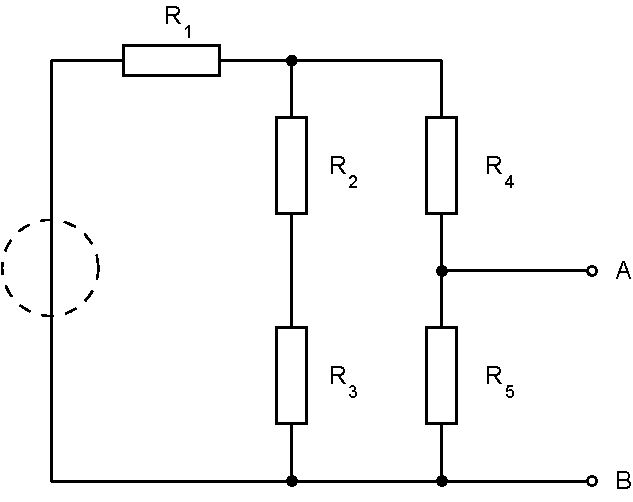
\includegraphics[scale=1,keepaspectratio]{xbednar00/zdroje/pr2/pr2_krok1.pdf}
\end{center}

\newpage
\subsection*{2. krok}
Spojíme sériovo zapojené zeristory $R_2$ a $R_3$.
\begin{center}
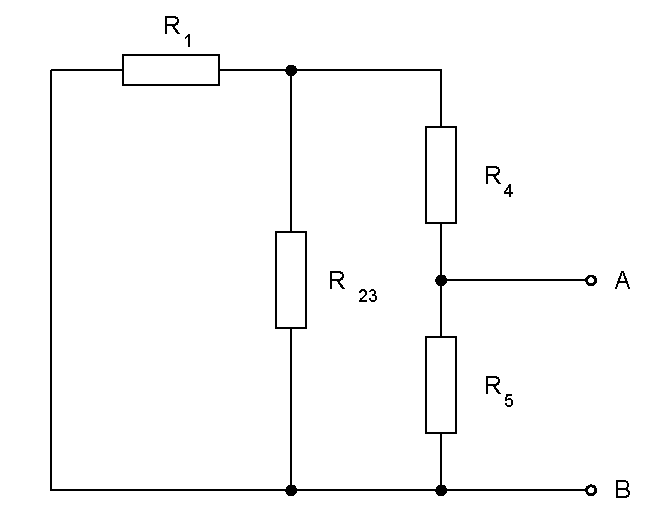
\includegraphics[scale=0.95,keepaspectratio]{xbednar00/zdroje/pr2/pr2_krok2.pdf}
\end{center}
$$R_{23}=R_2+R_3=850\Omega$$\\

\subsection*{3. krok}
Spojíme paralélne zapojené rezistoroy $R_1$ a $R_{23}$.
\begin{center}
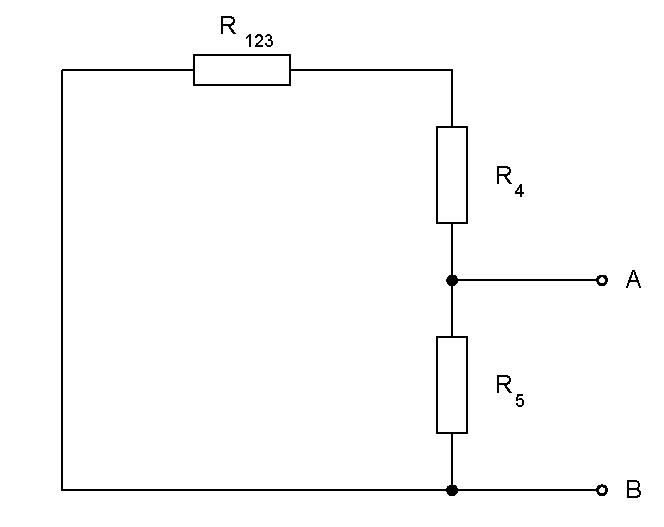
\includegraphics[scale=0.95,keepaspectratio]{xbednar00/zdroje/pr2/pr2_krok3.pdf}
\end{center}
$$R_{123}=\frac{R_1*R_{23}}{R_1+R_{23}}\doteq64,6739\Omega$$

\newpage
\subsection*{4. krok}
Spojíme sériovo zapojené  rezistory $R_{123}$ a $R_4$. Následne vypočítame $R_i$.
\begin{center}
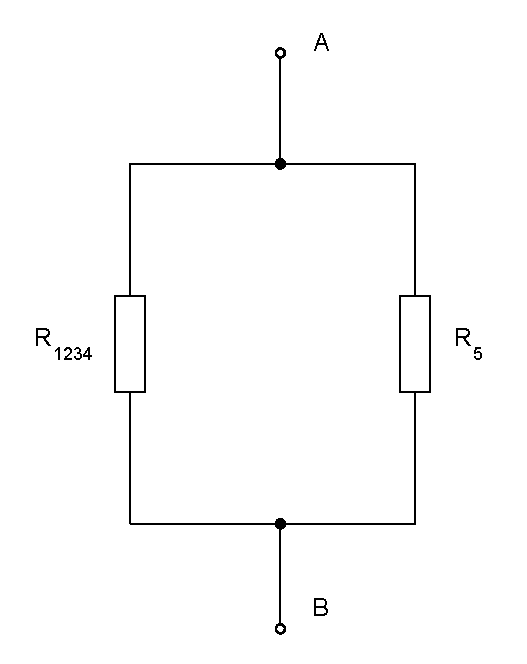
\includegraphics[scale=0.65,keepaspectratio]{xbednar00/zdroje/pr2/pr2_krok4.pdf}
\end{center}
$$R_{1234}=R_{123}+R_4\doteq304,6739\Omega$$
$$R_i=\frac{R_{1234}*R_5}{R_{1234}+R_5}\doteq161,6722\Omega$$

\subsection*{5. krok}
Vrátime sa k pôvodnej schéme a vypočítame $U_i$.
\begin{center}
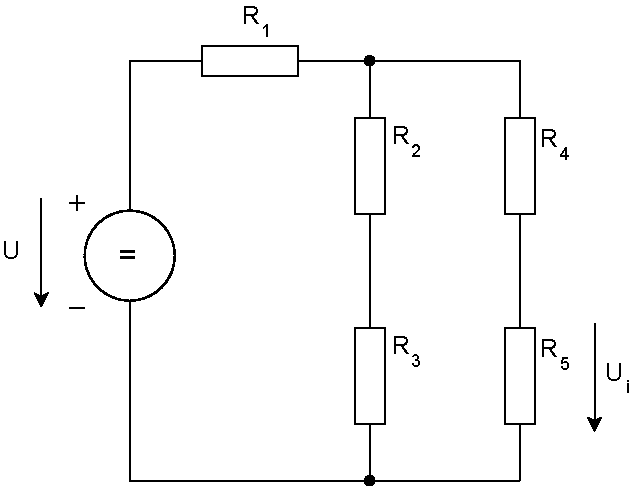
\includegraphics[scale=0.65,keepaspectratio]{xbednar00/zdroje/pr2/pr2_krok5.pdf}
\end{center}
$$R_{EKV}= R_1+\frac{R_{23}*R_{45}}{R_{23}+R_{45}} = R_1+\frac{(R_2+R_3)*(R_4+R_5)}{R_2+R_3+R_4+R_5} \doteq 450,8442\Omega$$
$$I = \frac{U}{R_{EKV}} \doteq 0,4436A$$
$$U_{R_1}+U_{R_{45}}-U = 0 \Longrightarrow U_{R_{45}} = U-U_{R_1} = U-I*R_1 \doteq 168,9471V$$
$$I_{R_{45}} = \frac{U_{R_{45}}}{R_{45}} \doteq 0,2449A$$
$$U_i = U_{R_5} = I_{R_{45}}*R_5 \doteq 110,1928V$$

\newpage
\subsection*{6. krok}
V náhradnom obvode dopočítame $\pmb{U_{R6}}$ a $\pmb{I_{R6}}$.
\begin{center}
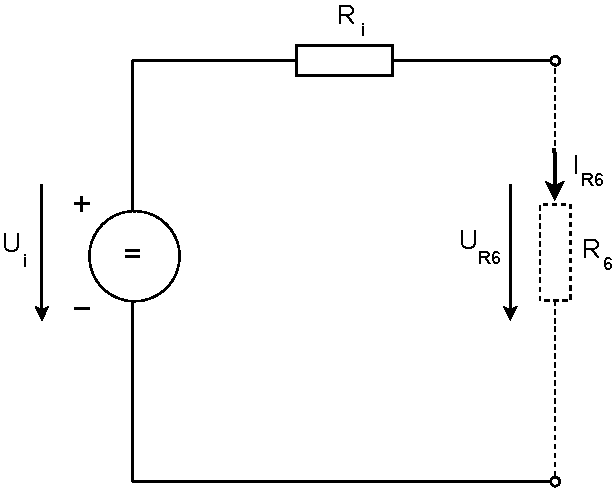
\includegraphics[scale=1,keepaspectratio]{xbednar00/zdroje/pr2/pr2_krok6.pdf}
\end{center}
$$\pmb{I_{R6}}= \frac{U_i}{R_i+R_6} \doteq \pmb{0,2887A}$$\\
$$\pmb{U_{R6}} = I_{R6}*R_6 \doteq \pmb{57,7369V}$$